
Here we present two examples of work, led by others, that has already been done making use of the models and ideas developed in chapters~\ref{ch:wake_models} and \ref{ch:wake_mapping}.
In the first, we apply the semi-analytic models to test the hypothesis that the kinematic arc detected in the disk of  HD~169142 is caused by a planet wake.
The second uses the linear wake theory to map the planet wake in the disk of IM Lupi through the peak velocity map from kinematic observations.

\section{The Kinematic Arc in HD~169142} \label{sec:hd169}

\textbf{Author Statement:} This section presents the semi-analytical modelling performed as a part of \citet{garg2022}, which is publicly available at \href{https://arxiv.org/abs/2207.02869}{\url{arXiv:2210.10248}}.
For this paper, I contributed the semi-analytic models used, advised the lead author on how to work with them, and provided feedback on the manuscript.

\subsection{Introduction}

HD~169142 is a disk-hosting Herbig Ae star located in the constellation of Sagittarius, at a distance of $117 \pm 4$ pc \citep{brown2016}.
The system's circumstellar disk appears almost face-on in the sky with an inclination of just $13^\circ$ \citep{raman2006,panic2008}.
The disk contains bright dust ring substructures at $\sim25$ au and $\sim65$ au, as well as a central cavity with radius $\sim22$ au.
These features have been observed through different tracers including scattered light \citep{quanz2013a,momose2015,pohl2017,bertrang2018} mid-infrared \citep{honda2012}, sub-millimetre with ALMA \citep{fedele2017,macias2019,perez2019} and centimetre with the Very Large Array \citep{osorio2014}.
The highest resolution of these studies showed that the outermost ring is actually three distinct rings separated by approximately $10$ au.
Various candidate point source detections have been made near the $r \approx 25$ au ring \citep{biller2014,reggiani2014,gratton2019}, but are disputed due to the possible confusion with disk material in their analyses \citep{ligi2018}.

This paper presents ALMA band 6 observations of the circumstellar disk around HD~169142.
We imaged the $^{12}$CO, $^{13}$CO and C$^{18}$O $J=2-1$ spectral lines at a resolution of $0.167 \, \mathrm{km/s}$, taking into account the Hanning Smoothing caused by the correlator.
The obtained angular resolutions of $0.07"$ and $0.1"$ allowed us resolve both density and kinematic substructures in the gas. Here, we will focus on the $^{12}$CO observations and on modelling the kinematics with the analytics.

\subsection{Observations and Analysis} \label{sec:obs_analysis_garg}

We imaged the $J=2-1$ line transitions of $^{12}$CO, $^{13}$CO and C$^{18}$O using ALMA band~6 observations from projects [2015.1.00490.S] and [2016.1.00344.S].
For details of the self-calibration and data reduction process, see \citet{garg2022}.

From equation \ref{eq:rot_eq_full}, the rotation velocity of the gas in a pressure-supported disk is given by 
\begin{align}
    \frac{v_{\rm gas}^2}{r} &= \frac{G M_\star r}{\left( r^2 + z^2  \right)^{3/2}} + \frac{1}{\rho_{\rm gas}} \partial_r P_{\rm gas}, \label{eq:gas_rotation}
\end{align}
where the first term is the typical Keplerian rotation and the second is the contribution by the radial pressure gradient.
As discussed in section \ref{sec:disk_rotation}, the second term typically results in sub-Keplerian motions.
To find kinematic substructures in the data, we wish remove the background motions of the disk associated with equation \ref{eq:gas_rotation} to isolate only the deviations from the bulk flow.
As a first step, we compute peak velocity $v_0$ maps by spectrally collapsing the data cube using the \textsc{Python} package \textsc{bettermoments} \citep{teague2018a}.
We chose specifically to use the \textit{Gaussian} method since it provides also the velocity error for each pixel $\delta v_0$ and has minimal statistical uncertainty \citep{yu2021}.

To obtain only the deviations from bulk rotation in $v_0$, we made use of the \textsc{Python} package \textsc{Eddy} \citep{teague2019}.
\textsc{Eddy} subtracts a best-fitting Keplerian rotation profile using a Markov Chain Monte Carlo (MCMC) method \citep{foreman-mackey2013}\footnote{The main point of using MCMC over a traditional optimisation methods is to obtain the uncertainties in the best fitting parameters by estimating the posterior distribution. However, we found that the error-bars we obtained were too small to be physically realistic, and so in appendix C of \citet{garg2022} we provide a parameter study around the best fit to investigate the true uncertainty.}.
We fit for the disk position angle (PA), central star mass $M_\star$, central star pixel location $(x_0,y_0)$ and systemic velocity $v_{\rm syst}$.
For the MCMC, we used 250 walkers and ran for 10,000 steps.
The data used in the fit were also restricted to within $1.5"$ from the centre of the image, as outside of this region was noise dominated.
The inner $0.2"$, equal to twice the beam width, was also exclude to avoid any bias resulting from beam smearing in the inner disk.
From fitting the $^{12}$CO data, we found best-fitting model parameters of $\mathrm{PA} = 5.33^\circ$, $M_\star = 1.47 \, \mathrm{M_\odot}$, and $v_{\rm syst} = 6.897 \, \mathrm{km/s}$.

To account for the pressure term of equation \ref{eq:gas_rotation}, we need the radial pressure gradient $\partial_r P_{\rm gas}(r)$.
Assuming an ideal gas equation of state, the pressure is given by 
\begin{align}
    P_{\rm gas}(r) = n_{\rm gas} k_{\rm B} T(r),
\end{align}
where $n_{\rm gas}$ is the gas number density, $k_{\rm B}$ is Boltzmann's constant and $T(r)$ is the temperature profile.
We calculated $n_{\rm gas}$ and $T(r)$ from the azimuthally averaged gas column density and brightness temperature profiles respectively, see \citet{garg2022} for further detail.

Finally, we made use of the best-fitting Keplerian rotation model, plus the radial pressure gradient, to subtract the bulk rotation from the peak velocity maps of the data to create kinematic residuals.
The result is shown in Figure \ref{fig:garg_arc}, along with the associated statistical significance.
We detect a kinematic excess of angular extent $\sim 105^\circ$ and magnitude $\sim 75 \, \mathrm{m/s}$ on the north side of the disk.
The excess is located between the $26$ au and $59$ au dust rings thus has a radial extent of approximately $30$ au.
The kinematic arc feature was however not detected in $^{13}$CO and C$^{18}$O, which may owe to the lower integration time of those observations, or may reflect that the rotation nearer to the mid-plane is less perturbed.

\begin{figure}
    \centering
    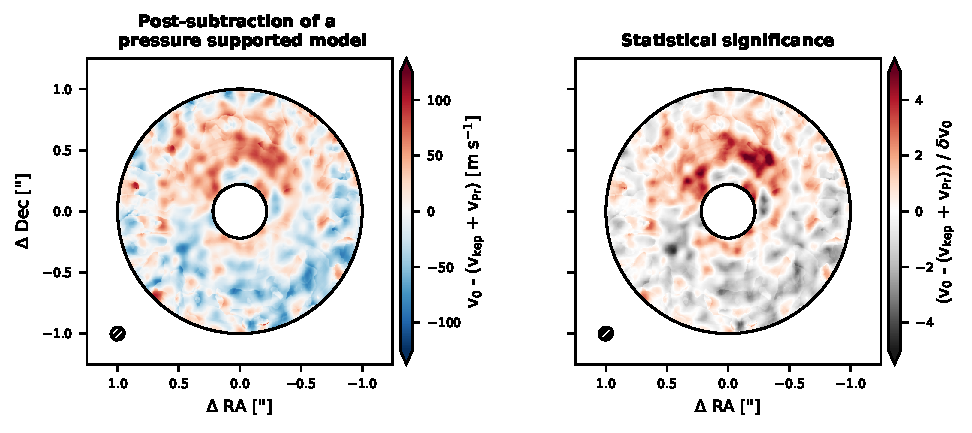
\includegraphics[width = 0.99\textwidth]{figures/garg_arc.pdf}
    \caption{Velocity residuals of the $^{12}$CO observations of HD~169142 calculated by the subtraction of a rotation profile including pressure support (left). Also shown is the residual velocities divided by the uncertainty in the peak velocity (right). The beam size is plotted in the bottom left corner of each panel, while the masked inner and outer regions are filled white \citep{garg2022}.}
    \label{fig:garg_arc}
\end{figure}

\subsection{Semi-Analytical Modelling} \label{sec:garg_analytics}

Notably, the feature we detected overlaps with the point source found in \citet{gratton2019} at a PA of $43.8^\circ$ and radial separation of $38$ au.
If the point source is a indeed a planet, perhaps the kinematic arc is associated with the velocity perturbations induced by the tidal forcing of the planet.
To test this scenario, we constructed semi-analytic models of the wake produced by a planet placed in the disk at the location of the \citet{gratton2019} point source using \textsc{wakeflow}.
We chose power law profiles for the unperturbed disk of $c \propto r^{-0.2}$ and $\Sigma \propto r^{-1}$, as well as an aspect ratio of $(H/r)_{\rm p}=0.08$.
The central star mass was chosen as $M_\star = 1.47 \, \mathrm{M_\odot}$ from the best-fitting model described in the previous section.
We used two $M_{\rm p}$ values of $1 \, \mathrm{M_J}$ and $10 \, \mathrm{M_J}$.

After the \textsc{wakeflow} models were calculated, we used the Monte Carlo radiation transfer code \textsc{mcfost} \citep{pinte2006,pinte2009} to generate synthetic $^{12}$CO $J=2-1$ observations.
The total gas mass of the model was set to $10^{-2} \, \mathrm{M_\odot}$ \citep{toci2019} and the gas-to-dust ratio was set to 100.
We use Mie theory \citep{mie1908} to calculate the optical properties of the dust grains, and assume that their size $a$ is distributed as $dn(a) \propto a^{-3.5} da$ where $n(a)$ is the number density of grains with size $a$.
The range of dust grain sizes used was between $0.03 \, \mathrm{\mu m}$ and $1$ mm, and they were taken to have a silicate composition \citep{weingartner2001}.
We assumed equal dust and gas temperatures, as well as local thermodynamic equilibrium.
The central star was modelled as an isotropically radiating blackbody, and $12.8\times 10^6$ packets were used to compute the dust temperature structure.
The relative CO abundance was taken to be $10^{-4}$, and the effects of CO freeze-out at $T < 20\, \mathrm{K}$, as well as photodissociation and photodesorption in regions of high UV were included \citep{pinte2018}.
The resultant channel maps had a channel spacing of $32 \, \mathrm{m/s}$, and the synthetic cubes were subsequently convolved spatially with a Gaussian of width $0.1"$ to replicate the beam size in the observations, as well as spectrally with a Hanning function of width $167 \, \mathrm{m/s}$ to replicate the effects of the correlator.

To create sky-plane velocity residuals, the cubes were collapsed spectrally in the same way as for the observations.
This whole process was then repeated except for models with no planet, and residuals were calculated as the different between the two velocity maps.
These residuals are presented in Figure \ref{fig:garg_analytics}.
Comparing these with Figure \ref{fig:garg_arc}, we see that in neither case do the analytic models recreate the arc found observationally.
The $1 \, \mathrm{M_J}$ planet model contains kinematic deviations that are far smaller than those observed.
On the other hand, the $10 \, \mathrm{M_J}$ produces residuals that while similar in amplitude, differ from the observations in shape, location and sign.
Of the two models, the $10 \, \mathrm{M_J}$ is more compatible with the observations but it still performs poorly.

Since the disk is nearly face-on, the observed kinematic structure may be dominated by vertical motions which are absent in the analytical models.
This may help to explain why the arc was absent in the $^{13}$CO and C$^{18}$O observations, since these trace the disk structure closer to the mid-plane.
For example, buoyancy spirals \citep{zhu2012,bae2021} excited by the planet in a thermally-stratified disk can result in significant vertical motions in the upper layers of the disk.
The planet wake in the mid-plane is expected to be dominated by radial motions \citep{rafikov2002a}, which would be hard to detect given the orientation of the disk.

A significant limitation to the analysis performed here is the accuracy of the \textsc{wakeflow} models nearby the planet.
Given the disk aspect ratio and central star mass, the thermal mass is only $\sim 0.5 \, \mathrm{M_J}$.
Thus the two models we have used here contain planets of masses $2 \, M_{\rm th}$ and $20 \, M_{\rm th}$.
In both of these cases the perturbations calculated close to the planet will be overestimated (\citeauthor{fasanoinprep.}, in prep.).
Unfortunately, in this case that is the region we are specifically interested in.
It is therefore only reasonable to interpret these results as upper bounds on the size of the perturbations that may be induced by the planet mass in each model.
We thus conclude that to explain the kinematic excess we have detected in the disk through our model requires a embedded planet of no more than $10 \, \mathrm{M_J}$.
%Planet masses were chosen based off the depth of the gas gap observed at $r=38$ au.
%Equation \ref{eq:kanagawa_gap_depth} relates the gap depth $\Sigma_{\rm p} / \Sigma_0$ to the aspect ratio $(H/r)_{\rm p}$, effective viscosity $\alpha$ and planet mass $M_{\rm p} / M_\star$.
%Taking our measured value of $\Sigma_{\rm p} / \Sigma_0 \approx 0.13$ in combination with  
%$(H/r)_{\rm p}=0.08$, and $\alpha=10^{-3}$ \citep{mulders2012,ansdell2018} gives an approximate planet mass of $\sim$
\begin{figure}
    \centering
    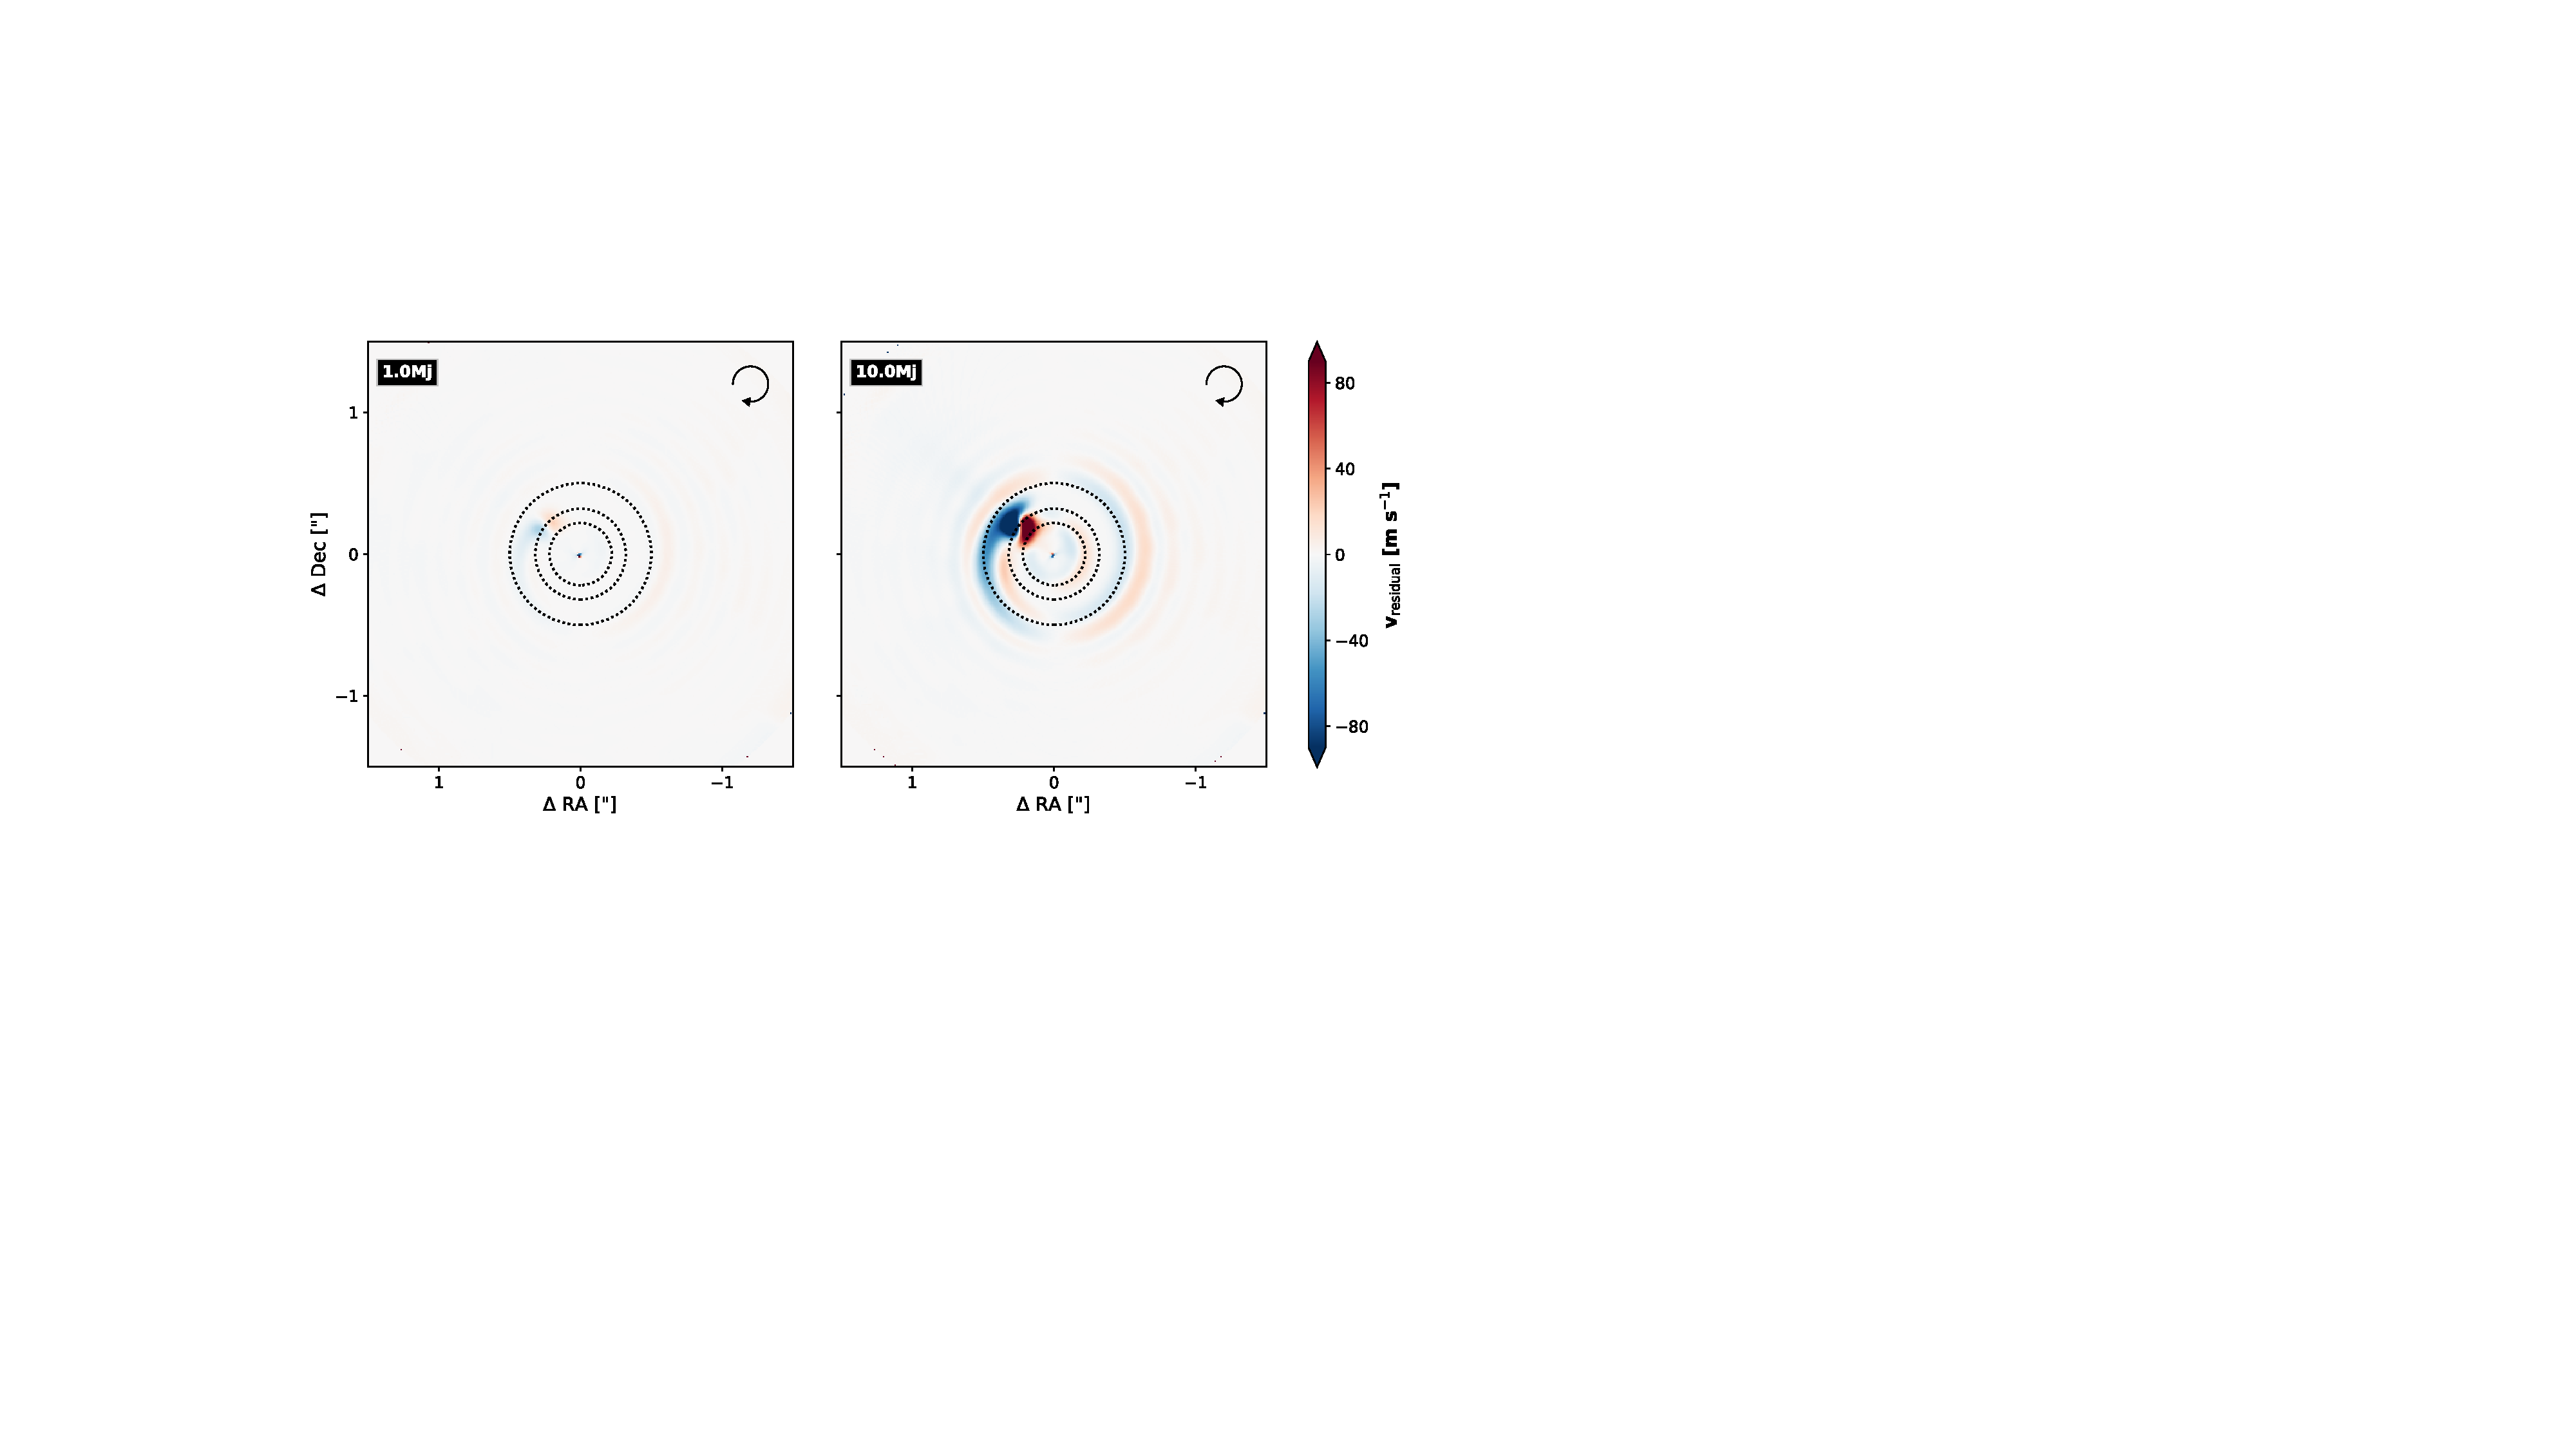
\includegraphics[width = 0.95\textwidth]{figures/garg_analytics_cw.pdf}
    \caption{Velocity perturbations from bulk rotation resulting from the tidal forcing of an embedded planet, calculated using \textsc{wakeflow} and \textsc{mcfost}. The $1 \, \mathrm{M_J}$ planet mass model is shown on the left, while the $10 \, \mathrm{M_J}$ model is shown on the right. The rotation direction of the disk is shown in the top-right of each panel \citep{garg2022}.}
    \label{fig:garg_analytics}
\end{figure}

\section{The Planet Wake in IM Lupi} \label{sec:IMLupiwake}

\textbf{Author Statement:} This section presents part of \citet{verrios2022}, which is publicly available at \href{https://arxiv.org/abs/2207.02869}{\url{arXiv:2207.02869}}.
For this paper, I provided the code used to create and project the wake shape to the emitting surface\footnote{\url{https://github.com/TomHilder/spiralmoments}}, created Figure~4 in collaboration with the lead author (Figure~\ref{fig:verrios_v0} here), and provided feedback on the manuscript.

\subsection{Introduction}

The young star IM~Lupi is host to a large and spectacular circumstellar disk \citep{panic2009,avenhaus2018,cleeves2016,pinte2018}.
Localised deviations from Keplerian motion were found across multiple velocity channels in $^{12}$CO line emission observations \citep{pinte2020} taken as part of DSHARP \citep{huang2018,andrews2018}.
Higher spatial resolution observations from MAPS \citep{oberg2021} confirm the presence of these velocity kinks, which \citet{pinte2020} hypothesised to be induced by the gravitational disturbance from an embedded planet orbiting at $117$ au.
This separation is too large to facilitate the detection of such a planet through traditional methods like radial velocities or transits, and the optically thick dust and gas material complicates direct imaging.

Scattered light images of the disk reveal large, tightly-wound spiral structures in the disk surface \citep[see Figure~\ref{fig:im_lup};][]{avenhaus2018},
while 1.25 mm continuum observations from DSHARP show also spiral arms and gaps in the dust-disk present in the mid-plane (see row 2 panel 1 of Figure~\ref{fig:maps_disks}; \citealt{huang2018}).
Are these spirals caused by the embedded protoplanet?
An alternative explanation is that they are formed through gravitational instabilities, which produce disordered flocculuent spirals and hence ``kinks everywhere'' \citep{hall2020}.
On the other hand, planets should produce velocity kinks only along the coherent one-armed planet wake.
The gravitational instability requires that the disk is self-gravitating and so massive, which is not required by the planet model.

In this letter we investigated whether an embedded planet can produce both the observed spiral structures and the observed kinematic features.
Here, we present the portion of the letter concerned with tracing the planet wake in the kinematics, similarly to in \citet{calcino2022}.

\subsection{Simulated Model}

We used the \textsc{phantom} SPH code \citep{price2018} to create models of the interaction between the disk of IM Lupi and an embedded planet.
A disk of mass $0.01 \, \mathrm{M_\odot}$ was modelled using ten million SPH particles, set to initially follow the density profile given in equation~\ref{eq:sigma_phantom}.
We used $p=0.48$ \citep{pinte2018} and $r_{\rm c}=150$ au.
We assumed a locally isothermal equation of state with $c \propto r^{-0.31}$, and a disk aspect ratio of $H/r=0.129$ at $r=100$ au.
The central star was modelled as a sink particle \citep{bate1995}, with a mass of $1.12 \, \mathrm{M_\odot}$ \citep{andrews2018} and an accretion radius of $1$ au.
We included dust in the simulations using the \textsc{multigrain} one-fluid algorithm \citep{price2015,ballabio2018,hutchison2018,price2018}.
We used 11 distinct grain sizes, logarithmically spaced between $a_{\rm min}=1.0 \, \mathrm{\mu m}$ and $a_{\rm max}=2300 \, \mathrm{\mu m}$ and following a distribution given by $dn(a) \propto a^{-3.5} \, da$.
The gas to dust ratio was set as $57$ resulting in a total dust mass of $1.7 \times 10^{-3} \, \mathrm{M_\odot}$ following \citep{pinte2018}. 

The planet was modelled as a non-accreting sink particle with a softened gravitational potential, following a procedure similar to that in \citet{szulagyi2016}.
This was done to minimise the fast migration and large mass growth that an accreting particle would experience due to the large number of SPH particles.
We performed simulations with varying planet masses of $2, \, 3, \, 5$ and $7\, \mathrm{M_J}$, although we will only discuss the $2 \, \mathrm{M_J}$ model here.

Radiation transfer was then performed on the SPH models using \textsc{mcfost} \citep{pinte2006,pinte2009} following a similar method to that outlined in sections~\ref{sec:garg_analytics} and \ref{sec:calcino_hydro}.
Refer to \citet{verrios2022} for further detail.

\subsection{Tracing the Wake}

\begin{figure}
    \centering
    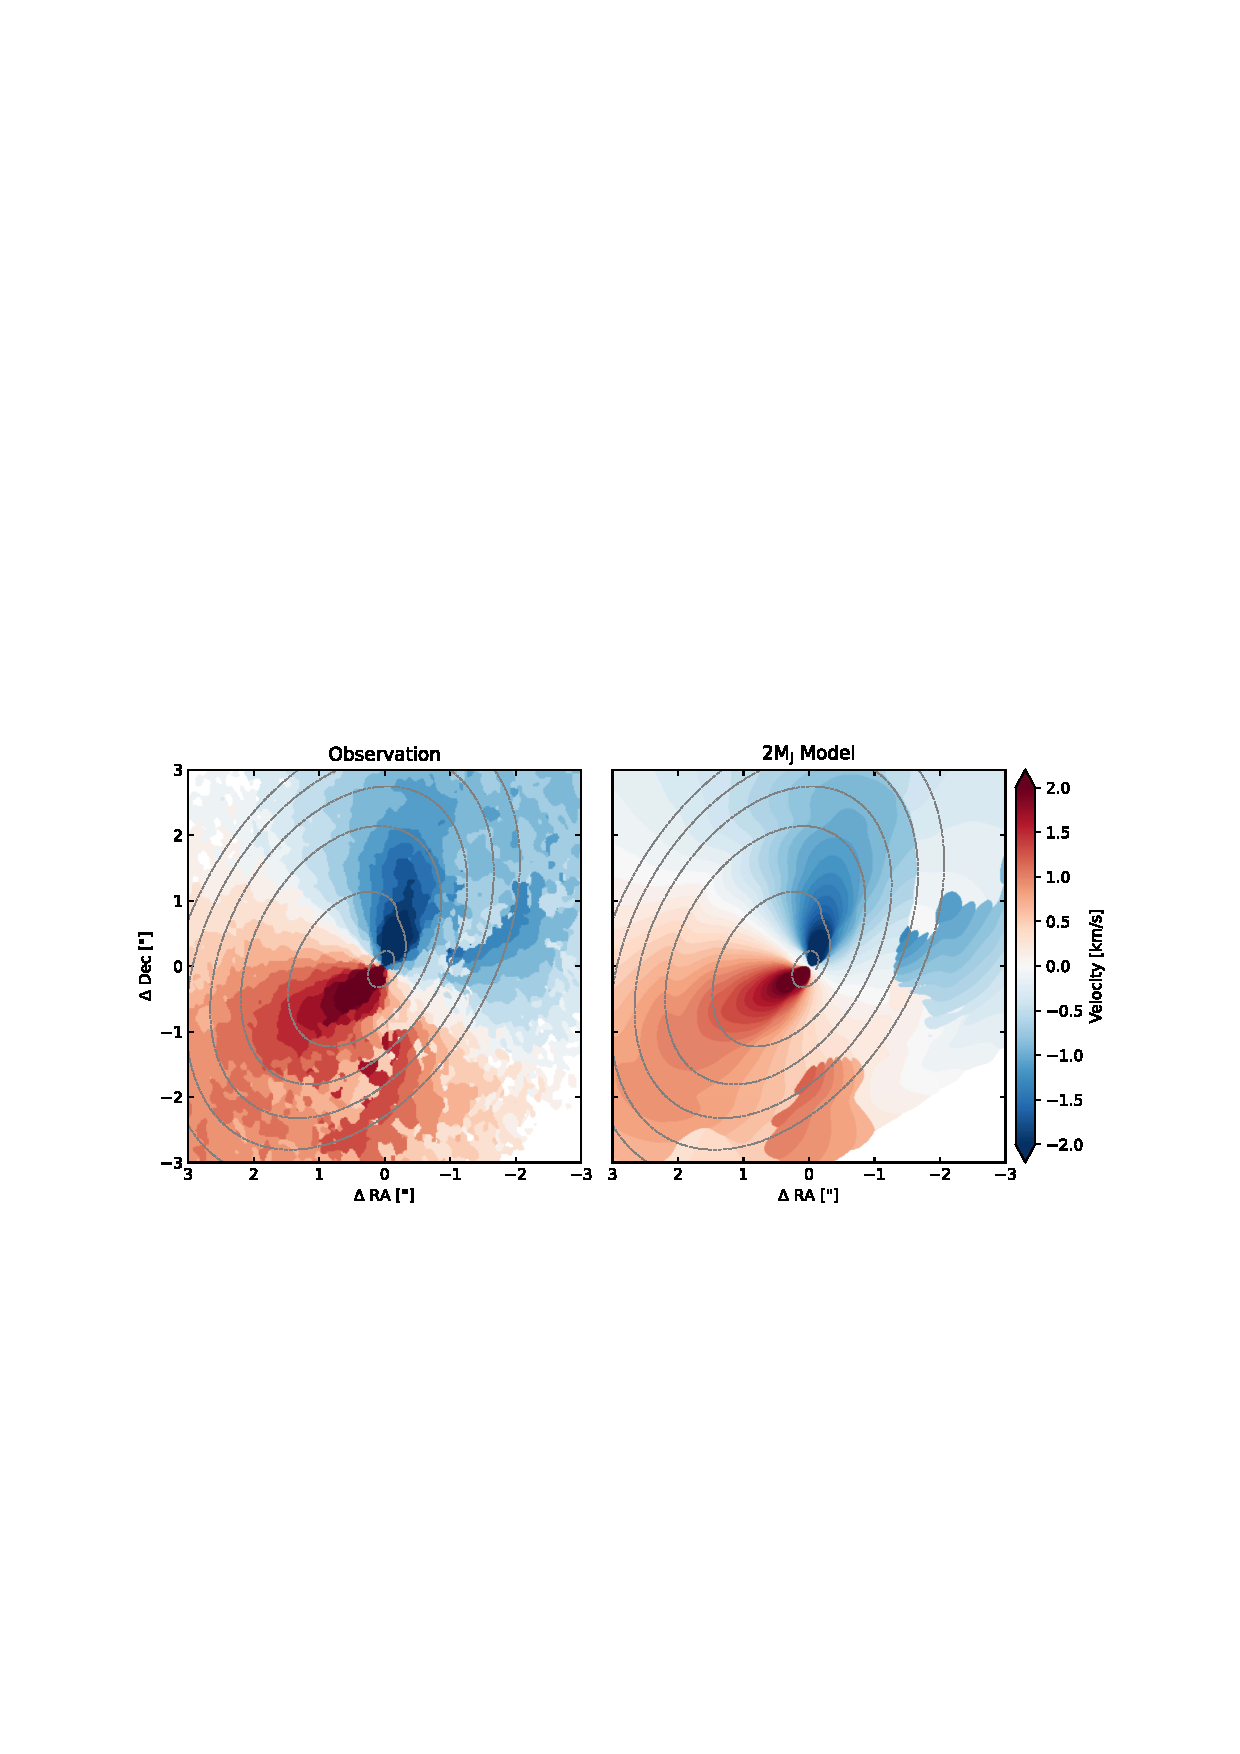
\includegraphics[width = 0.99\textwidth]{figures/verrios_v0.pdf}
    \caption{The left panel shows the peak velocity map of the $^{12}$CO line emission data from MAPS \citep{oberg2021}. The right panel shows the analogous synthetic map produced with our $2 \, \mathrm{M_J}$ model. The dotted line in both panels shows the expected location of the planet wake as predicted by linear theory \citep{ogilvie2002}, projected to the top emitting surface of the disk \citep{pinte2018,law2021}.}
    \label{fig:verrios_v0}
\end{figure}

A key prediction of the embedded planet hypothesis is that the one-armed planet wake excited by the planet should create velocity kinks any time it intersects a velocity channel.
\citet{calcino2022} found that this may be used to trace the planet wake shape through kinematic observations.
The presence of a coherent planet wake in the observations would provide evidence for the embedded planet model over gravitational instability.
\citet{calcino2022} also found that the wake is best traced in the peak velocity map.

Were therefore use spectrally collapsed both the MAPS $^{12}$CO observations \citep{oberg2021} and the synthetic observations from our SPH + radiation transfer model to create peak velocity maps.
These are plotted in Figure~\ref{fig:verrios_v0}, with the data shown in the left panel, and the model in the right.
We additionally calculated the expected wake shape using equation \ref{eq:power_law_wake} \citep{ogilvie2002,rafikov2002a}, and projected it to the emission surface determined by \citet{law2021a} following the method of \citet{calcino2022}.
This is shown in both panels (grey dashed line).
The velocity perturbations, which manifest as distorted contours, are seen to trace the planet wake shape through the outer disk in both the model and the observations.
The are particularly obvious in the second passage of the outer wake in the north side of the disk.
In addition, the ``N-wave'' structure predicted by the semi-analytic models (\citealt{goodman2001}; \citealt{rafikov2002a}; \citetalias{bollati2021}) can be seen in the observations in the same region.

We therefore confirm that the wake from the planet is visible in the peak velocity map of the $^{12}$CO observations, as predicted by the embedded planet model.